%%%%%%%%%%%%%%%%%%%%%%%%%%%%%%%%%%%%%%%%%
% HW Template
% LaTeX Template
% Version 1.0 (19/10/18)
% Modified by
% Erdem TUNA
% Halil TEMURTAŞ 
% Enes TAŞTAN 
%%%%%%%%%%%%%%%%%%%%%%%%%%%%%%%%%%%%%%%%%
%
%----------------------------------------------------------------------------------------
%	PACKAGES AND OTHER DOCUMENT CONFIGURATIONS
%----------------------------------------------------------------------------------------
\documentclass[a4paper,12pt]{article}
%-----packages------
\usepackage[a4paper, total={6.2in, 8.5in}]{geometry}
\usepackage[english]{babel}
\usepackage[utf8x]{inputenc}
\usepackage{amsmath}
\usepackage{graphicx}
\usepackage[colorinlistoftodos]{todonotes}
\usepackage{gensymb} % this could be problem
\usepackage{float}
\usepackage{fancyref}
\usepackage{subcaption}
\usepackage[toc,page]{appendix} %appendix package
\usepackage{xcolor}
\usepackage{listings}
\usepackage{xspace}
\usepackage{amssymb}
\usepackage{nicefrac}
\usepackage{gensymb}
\usepackage{fancyhdr}
\usepackage{blindtext}  % for dummy text, use \blindtext or \BlindText
\usepackage{lipsum}    % for dummy text, use \lipsum[3-56]
\usepackage[final]{pdfpages}  % pdf include
\usepackage{array} %allows more options in tables
\usepackage{pgfplots,pgf,tikz} %coding plots in latex
\usepackage{capt-of} % allows caption outside the figure environment
\usepackage[export]{adjustbox} %more options for adjusting the images
\usepackage{multicol,multirow,slashbox} % allows tables like table1
%\usepackage[hyperfootnotes=false]{hyperref} % clickable references
\usepackage{epstopdf} % useful when matlab is involved
%\usepackage{placeins} % prevents the text after figure to go above figure with \FloatBarrier 
%\usepackage{listingsutf8,mcode} %import .m or any other code file mcode is for matlab highlighting
\usepackage{enumitem}
\usepackage{hyperref}

%-----end of packages

%-----specifications-----
\definecolor{mGreen}{rgb}{0,0.6,0} % for python
\definecolor{mGray}{rgb}{0.5,0.5,0.5}
\definecolor{mPurple}{rgb}{0.58,0,0.82}
\definecolor{mygreen}{RGB}{28,172,0} % color values Red, Green, Blue for matlab
\definecolor{mylilas}{RGB}{170,55,241}

\setcounter{secnumdepth}{5} % how many sectioning levels to assign numbers to
\setcounter{tocdepth}{5}    % how many sectioning levels to show in ToC

\lstdefinestyle{CStyle}{
	commentstyle=\color{mGreen},
	keywordstyle=\color{magenta},
	numberstyle=\tiny\color{mGray},
	stringstyle=\color{mPurple},
	basicstyle=\footnotesize,
	breakatwhitespace=false,         
	breaklines=true,
	frame=single,
	rulecolor=\color{black!40},                 
	captionpos=b,                    
	keepspaces=true,                 
	numbers=left,                    
	numbersep=5pt,                  
	showspaces=false,                
	showstringspaces=false,
	showtabs=false,                  
	tabsize=2,
	language=C
}

\lstset{language=Matlab,%
	%basicstyle=\color{red},
	breaklines=true,%
	frame=single,
	rulecolor=\color{black!40},
	morekeywords={matlab2tikz},
	keywordstyle=\color{blue},%
	morekeywords=[2]{1}, keywordstyle=[2]{\color{black}},
	identifierstyle=\color{black},%
	stringstyle=\color{mylilas},
	commentstyle=\color{mygreen},%
	showstringspaces=false,%without this there will be a symbol in the places where there is a space
	numbers=left,%
	numberstyle={\tiny \color{black}},% size of the numbers
	numbersep=9pt, % this defines how far the numbers are from the text
	emph=[1]{for,end,break},emphstyle=[1]\color{red}, %some words to emphasise
	%emph=[2]{word1,word2}, emphstyle=[2]{style},    
}


\tikzset{
	desicion/.style={
		diamond,
		draw,
		text width=4em,
		text badly centered,
		inner sep=0pt
	},
	block/.style={
		rectangle,
		draw,
		text width=10em,
		text centered,
		rounded corners
	},
	cloud/.style={
		draw,
		ellipse,
		minimum height=2em
	},
	descr/.style={
		fill=white,
		inner sep=2.5pt
	},
	connector/.style={
		-latex,
		font=\scriptsize
	},
	rectangle connector/.style={
		connector,
		to path={(\tikztostart) -- ++(#1,0pt) \tikztonodes |- (\tikztotarget) },
		pos=0.5
	},
	rectangle connector/.default=-2cm,
	straight connector/.style={
		connector,
		to path=--(\tikztotarget) \tikztonodes
	}
}

\tikzset{
	desicion/.style={
		diamond,
		draw,
		text width=4em,
		text badly centered,
		inner sep=0pt
	},
	block/.style={
		rectangle,
		draw,
		text width=10em,
		text centered,
		rounded corners
	},
	cloud/.style={
		draw,
		ellipse,
		minimum height=2em
	},
	descr/.style={
		fill=white,
		inner sep=2.5pt
	},
	connector/.style={
		-latex,
		font=\scriptsize
	},
	rectangle connector/.style={
		connector,
		to path={(\tikztostart) -- ++(#1,0pt) \tikztonodes |- (\tikztotarget) },
		pos=0.5
	},
	rectangle connector/.default=-2cm,
	straight connector/.style={
		connector,
		to path=--(\tikztotarget) \tikztonodes
	}
}
%-----end of specifications-----


%----commands----
\newcommand\nd{\textsuperscript{nd}\xspace}
\newcommand\rd{\textsuperscript{rd}\xspace}
\newcommand\nth{\textsuperscript{th}\xspace} %\th is taken already
\newcommand{\specialcell}[2][c]{ \begin{tabular}[#1]{@{}c@{}}#2\end{tabular}} % for too long table lines

\newcommand{\blankpage}{
	\- \\[9cm]	
	{ \centering \textit{This page intentionally left blank.} \par }
	\- \\[9cm]
}% For Blank Page

\makeatletter
\renewcommand\paragraph{\@startsection{paragraph}{4}{\z@}%
	{-2.5ex\@plus -1ex \@minus -.25ex}%
	{1.25ex \@plus .25ex}%
	{\normalfont\normalsize\bfseries}}
\makeatother
%-----end of commands-----

\pagestyle{fancy}
\fancyhead[LO,LE]{Halil TEMURTAŞ / 2094522 }
\fancyhead[RO,RE]{December 17, 2018}
\fancyfoot[RO,RE]{
\includegraphics[width=2.7cm]{images/eelogo}}

\begin{document}
\begin{center}
	\textbf{\large EE407 Process Control \\[0.2cm] Experiment 3} \\
\end{center}


	\begin{enumerate}
		\item From conservation law
			
			$$ q_in(t)-q_{out}(t)=\frac{d(Volume)}{dt} $$
			
			$$ q_in(t)-q_{out}(t)=A \frac{dh(t)}{dt} $$
			
			$$\boxed{ \frac{dh(t)}{dt}+ \frac{1}{A}\frac{h(t)}{R}\ =\ \frac{1}{A} q_in(t) }$$
		
		
		\item Taking the Laplace Transform of the both side
		
			$$ [s+\frac{1}{AR}]\ H(s)=\frac{1}{A}Q_i(s) $$

			$$\boxed{ G(s)=\frac{H(s)}{Q_i(s)}=\frac{AR}{A(sAR+1)} }$$		
		
		\item The block diagram of the Figure 5 from Preliminary Work can be seen at \textit{Figure~\ref{fig:block}} while of the Figure 6 from Preliminary Work can be seen at \textit{Figure~\ref{fig:withcontr}}.
		
			\begin{figure}[H]
				\center
				\setlength{\unitlength}{\textwidth} 
				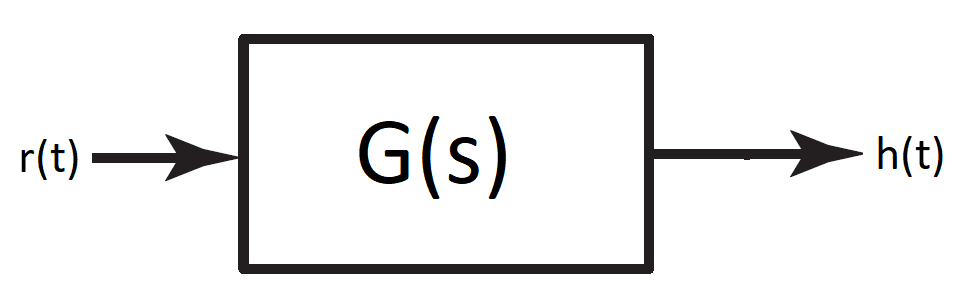
\includegraphics[width=0.5\unitlength]{images/block}
				\caption{\label{fig:block} Block Diagram of the Open-Loop System }
			\end{figure}
				
			\begin{figure}[H]
				\center
				\setlength{\unitlength}{\textwidth} 
				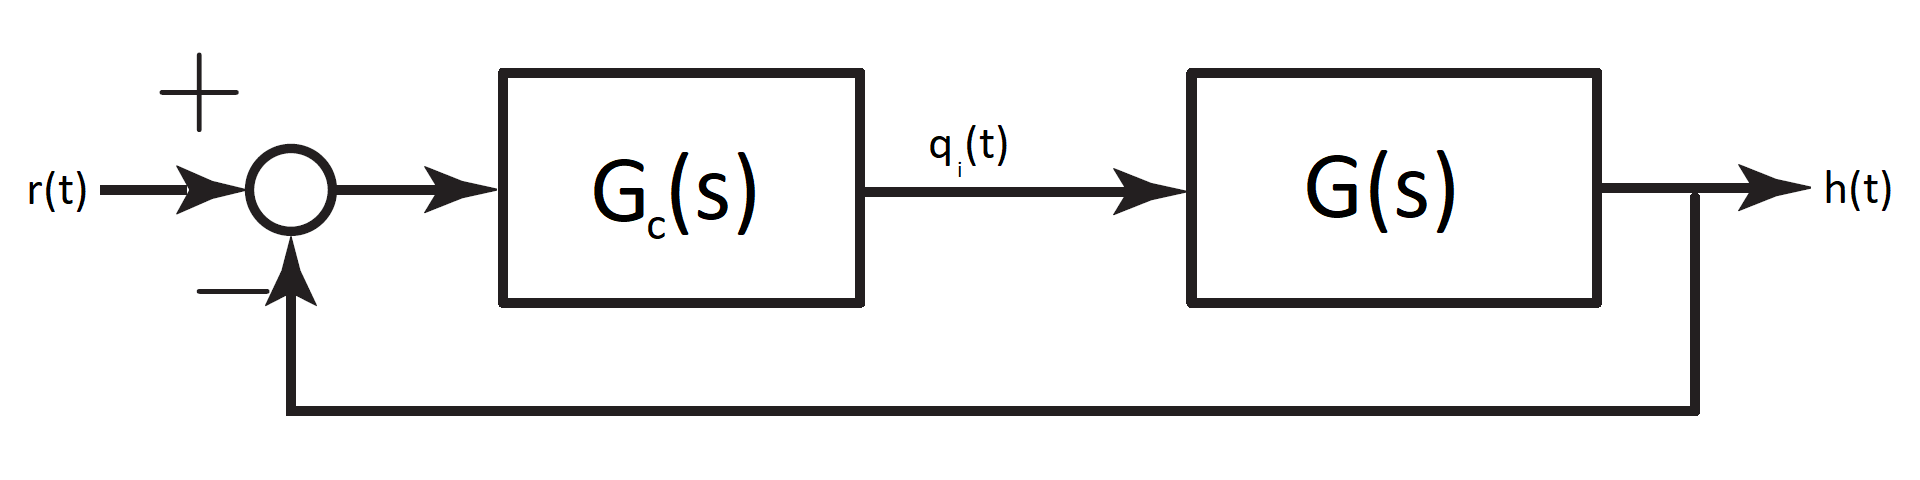
\includegraphics[width=0.8\unitlength]{images/withcontr}
				\caption{\label{fig:withcontr} Block Diagram of the Closed-Loop System }
			\end{figure}
		
		
			General closed loop transfer function of the closed-loop system can be found to be as;
			
			$$G_{CL}(s)=\frac{G_c(s)G(s)}{1+G_c(s)G(s)}$$
			\begin{enumerate}
				
			
				
				\item 
				
					$$ G_c(s)= KL^{-1} $$
					
					$$ G_{CL}(s)=\cfrac{(KL^{-1})(\cfrac{AR}{A(sAR+1)})}{1+(KL^{-1})(\cfrac{AR}{A(sAR+1)})} = \cfrac{ARKL^{-1}}{A(sAR+1)+ARKL^{-1}}$$
					
					$$\boxed{ 	G_{CL}(s)= \frac{ARKL^{-1}}{sA^2R+A+ARKL^{-1}} }$$ 
					
					
						
				
				\item 
				
					$$ G_c(s)= KL^{-1}(1+\frac{1}{T_1s}+\frac{T_2s}{1+aT_2s})$$
					
					$$\boxed{ G_{CL}(s)=\cfrac{KL^{-1}(1+\cfrac{1}{T_1s}+\cfrac{T_2s}{1+aT_2s})\cfrac{AR}{A(sAR+1)}}{1+KL^{-1}(1+\cfrac{1}{T_1s}+\cfrac{T_2s}{1+aT_2s})\cfrac{AR}{A(sAR+1)}} }$$
					
					
			\end{enumerate}
		
		
		\item Offset at the output can be found from final value theorem
			
			$$ y_{ss}=\lim_{s \to 0}sY(s) = \lim_{s \to 0}sG_{CL}(s)R(s)$$
			
			Assuming step input for simplicity
			
			$$ y_{ss} = \lim_{s \to 0} \frac{G_c(s)G(s)}{1+G_c(s)G(s)}$$
			
			For P-Controller
			
				$$ 	\lim_{s \to 0} G_c(s)=K_p=KL^{-1} $$			
				
				$$ \lim_{s \to 0} G(s)=\frac{AR}{A}=R $$
				
				$$ y_{ss}= \frac{RKL^{-1}}{1+RKL^{-1}} $$
					
				Thus, the offset can be found as follows;
				
				$$\boxed{ offset\ =\ e_{ss}= 1-y_{ss}=1- \frac{RKL^{-1}}{1+RKL^{-1}} }$$
				
		\item For PI-Controller
			
			$$ 	\lim_{s \to 0} G_c(s) \to \infty $$			
				
			$$ \lim_{s \to 0} G(s)=\frac{AR}{A}=R $$
				
			$$ e_{ss} \to 0 $$
				
			Thus, the offset can be found as zero.
				
			The pole at the origin due to integral term of the PI controller makes the steady state error zero. The integral term can make system oscillatory or even drive system to unstable region.


		\item The noises at the closed loop system can easily be amplified by the derivative component of the controller. To avoid this, alternative variables which can replace the derivative of the processed variable can be used. For example, in a case where the distance is the PV, the controller can use an alternate variable such as \textbf{speed} instead of derivative action. Such alternate controllers to PD controllers is called \textbf{PV Controllers}.
	\end{enumerate}
		
					

		
		

	
%\begin{appendices}
%\section{Source Code for Matlab Part}\label{appendix}
	%%	\lstinputlisting[language=Matlab,firstline=33, lastline=34]{q13.m} \-\\[1cm]		
%\lstinputlisting[language=Matlab]{Exp4.m} 
%\end{appendices}


\end{document}

%----samples------
%\begin{itemize}
%\item Item
%\item Item
%\end{itemize}

%\begin{figure}[H]
%\center
%\setlength{\unitlength}{\textwidth} 
%\includegraphics[width=0.7\unitlength]{images/logo1}
%\caption{\label{fig:logo}Logo }
%\end{figure}

%\begin{figure}[H]
%	\setlength{\unitlength}{\textwidth} 
%	\centering
%	\begin{subfigure}{.5\textwidth}
%  		\centering
%  		\includegraphics[width=0.48\unitlength]{images/logo1}
%  		\caption{\label{fig:logo1}Logo1 }
%	\end{subfigure}%
%	\begin{subfigure}{.5\textwidth}
%  		\centering
%		\includegraphics[width=0.48\unitlength]{images/logo2}
%  		\caption{\label{fig:logo2}Logo2}
%	\end{subfigure}
%\caption{\label{fig:calisandegree} Small Logos   }
%\end{figure}
	
%\begin{table}[H]
%  \centering
% 
%    \begin{tabular}{c|c|c}
%       $$A$$ & $$B$$ & $$C$$ \\ \hline
%       1 & 2 & 3  \\ \hline
%       2 & 3 & 4  \\ \hline
%       3 & 4 & 5  \\ \hline
%       4 & 5 & 6  
%      
%  \end{tabular}
%  \caption{table}
%  \label{tab:table}
%\end{table}
	
%\begin{table}[H]
%  \centering
% 
%    \begin{tabular}{c|c|c}
%       \backslashbox{$A$}{$a$} & $$\specialcell{ Average deviation \\ after subtracting out the  \\ frequency error }$$ & $$C$$ \\ \hline
%       \multirow{2}{*}{1} & 2 & 3  \\ \cline{2-3}
%        & 3 & 4  \\ \hline
%       3 & \multicolumn{2}{c}{4}  \\ \hline
%       4 & 5 & 6  
%      
%  \end{tabular}
%  \caption{table}
%  \label{tab:table}
%\end{table}
%-----end of samples-----